\section*{Chapter 3}

\subsection*{Exercise 3.1}
Devise three example tasks of your own that fit into the MDP framework,
identifying for each its states, actions, and rewards. Make the three examples as different
from each other as possible. The framework is abstract and flexible and can be applied in
many different ways. Stretch its limits in some way in at least one of your examples.

\subsubsection*{Solution:}
Example 1: Chess Player Program\\
Task Description: A chess-playing program aims to play chess in a way that conceals its identity as a non-human player.

\begin{itemize}
    \item \textbf{States (S):}
    \begin{itemize}
        \item Current board position (the arrangement of pieces).
        \item Time remaining for each player.
        \item Opponent's previous move history.
    \end{itemize}
    
    \item \textbf{Actions (A):}
    \begin{itemize}
        \item Make a legal move
        \item Pause (to simulate human behavior, potentially to analyze).
        \item Offer a draw or resignation.
    \end{itemize}
    
    \item \textbf{Rewards (R):}
    \begin{itemize}
        \item +1 for winning the game.
        \item -1 for drawing or losing.
        \item -0.01 for making moves that are too optimal, which might reveal the program's identity (e.g., moving in a way that a human wouldn't).
        \item +0.01 for making "human-like" moves (less optimal but more deceptive).
    \end{itemize}
\end{itemize}

Example 2: Person Taking an IQ Test\\
Task Description: A person takes an IQ test with the goal of maximizing their score.

\begin{itemize}
    \item \textbf{States (S):}
    \begin{itemize}
        \item Current question number.
        \item The question itself.
        \item Time left for the test.
    \end{itemize}
    
    \item \textbf{Actions (A):}
    \begin{itemize}
        \item Answer the question (select one of multiple-choice options).
        \item Think.
        \item Skip the question.
    \end{itemize}
    
    \item \textbf{Rewards (R):}
    \begin{itemize}
        \item +1 for a correct answer.
        \item 0 for a skipped question.
        \item -1 for an incorrect answer.
    \end{itemize}
\end{itemize}

Example 3: Elevator Control System\\
Task Description: An elevator system optimizes its operation to minimize wait times and maximize efficiency in a multi-story building.

\begin{itemize}
    \item \textbf{States (S):}
    \begin{itemize}
        \item Current floor of the elevator.
        \item Status of the elevator (moving up, moving down, idle).
        \item Status of the door (open, closed)
        \item Floors where people wish to go up.
        \item Floors where people wish to go down.
        \item Current load (number of passengers in the elevator based on weight).
        \item Buttons pressed (which floors the passengers in the elevator wish to go to).
    \end{itemize}
    
    \item \textbf{Actions (A):}
    \begin{itemize}
        \item Move up.
        \item Move down.
        \item Open doors.
        \item Close doors.
        \item Wait on the current floor.
    \end{itemize}
    
    \item \textbf{Rewards (R):}
    \begin{itemize}
        \item -1 for each second the passengers spend waiting.
        \item -1 for unnecessary movements (e.g., moving to a floor with no waiting passengers).
    \end{itemize}
\end{itemize}


\subsection*{Exercise 3.2}
Is the MDP framework adequate to usefully represent all goal-directed learning tasks? Can you think of any clear exceptions?

\subsubsection*{Solution:}
There are situations where the MDP framework is not adequate. 
\begin{itemize}
    \item Continous action spaces
    \item Non-Markovian environments
    \item High-Dimensional state spaces
\end{itemize}

Example: self-driving for cars have continous action spaces (steering the wheel, rate of acceleration) and high-dimensional state spaces (images of the environment).

\subsection*{Exercise 3.3}
Consider the problem of driving. You could define the actions in terms of
the accelerator, steering wheel, and brake, that is, where your body meets the machine.
Or you could define them farther out—say, where the rubber meets the road, considering
your actions to be tire torques. Or you could define them farther in—say, where your
brain meets your body, the actions being muscle twitches to control your limbs. Or you
could go to a really high level and say that your actions are your choices of where to drive.
What is the right level, the right place to draw the line between agent and environment?
On what basis is one location of the line to be preferred over another? Is there any
fundamental reason for preferring one location over another, or is it a free choice?

\subsubsection*{Solution:} 
The right place to draw the line between agent and environment is highly dependant on the problem we are modeling/trying to solve. If we want to create a route finding algorithm, then the highest level of choice would be ideal, but if we want to look at the problem in a neuroscientific way, then the brain and muscle option would be fine.\\
There is no fundamental reason for preferring one location over another, it is only good for using the advantages of abstraction.


\subsection*{Exercise 3.4}
Give a table analogous to that in Example 3.3, but for $p(s', r |s, a)$ . It
should have columns for $s$, $a$, $s'$, $r$, and $p(s', r |s, a)$ , and a row for every 4-tuple for which
$p(s', r |s, a)  > 0$.

\subsubsection*{Solution:}

\begin{table}[h!]
    \centering
    \begin{tabular}{ll|ll|c}
        $s$  & $a$      & $s'$ & $r$                 & $p(s', r |s, a)$ \\ \hline
        high & search   & high & $r_{\text{search}}$ & $\alpha$         \\
        high & search   & low  & $r_{\text{search}}$ & $1 - \alpha$     \\
        low  & search   & high & -3                  & $1 - \beta$      \\
        low  & search   & low  & $r_{\text{search}}$ & $\beta$          \\
        high & wait     & high & $r_{\text{wait}}$   & 1                \\
        low  & wait     & low  & $r_{\text{wait}}$   & 1                \\
        low  & recharge & high & 0                   & 1               
    \end{tabular}
\end{table}


\subsection*{Exercise 3.5}
The equations in Section 3.1 are for the continuing case and need to be
modified (very slightly) to apply to episodic tasks. Show that you know the modifications
needed by giving the modified version of (3.3).

\subsubsection*{Solution:}
The original equation:
\[
\sum_{s' \in S} \sum_{r \in R} P(s', r \mid s, a) = 1, \quad \forall s \in S, \forall a \in A(s)
\]

This would exclude the terminal states $S^+ \setminus S$, so we wouldn't count the cases where a state goes from non-terminal to a terminal state.

The modified equation:
\[
\sum_{s' \in S^+} \sum_{r \in R} P(s', r \mid s, a) = 1, \quad \forall s \in S^+, \forall a \in A(s)
\]


\subsection*{Exercise 3.6}
Suppose you treated pole-balancing as an episodic task but also used
discounting, with all rewards zero except for  1 upon failure. What then would the
return be at each time? How does this return differ from that in the discounted, continuing
formulation of this task?

\subsubsection*{Solution:}

\[
G_t = \sum_{k=0}^{T-t} \gamma^k r_{t+k+1} = 0 + 0 + 0 + \dots + -\gamma^{T-t} = -\gamma^{T-t}
\]

The reward in the discounted, continuing formulation:

\[
G_t = \sum_{k \in K} -\gamma^{k-t}
\]

Where $K$ is the number of time steps before failure (as well as to the times of later failures).


\subsection*{Exercise 3.7} Imagine that you are designing a robot to run a maze. You decide to give it a
reward of +1 for escaping from the maze and a reward of zero at all other times. The task
seems to break down naturally into episodes—the successive runs through the maze—so
you decide to treat it as an episodic task, where the goal is to maximize expected total
reward (3.7). After running the learning agent for a while, you find that it is showing
no improvement in escaping from the maze. What is going wrong? Have you effectively
communicated to the agent what you want it to achieve?

\subsubsection*{Solution:}

The agent receives +1 reward regardless of the timesteps it takes it to leave the maze. Because of this, it can't distinguish a good policy from a bad one.

\subsection*{Exercise 3.8}
Suppose $\gamma = 0.5$ and the following sequence of rewards is received $R_1 = -1$, $R_2 = 2$, $R_3 = 6$, $R_4 = 3$, and $R_5 = 2$, with $T = 5$. What are $G_0$, $G_1$, $\dots$, $G_5$? Hint:
Work backwards.

\subsubsection*{Solution:}

\begin{equation}
    \begin{aligned}
        G_t &= R_{t+1} + \gamma G_{t+1} \\
        G_5 &= 0 \\
        G_4 &= 2 + 0.5 \cdot 0 = 2 \\
        G_3 &= 3 + 0.5 \cdot 2 = 4 \\
        G_2 &= 6 + 0.5 \cdot 4 = 8 \\
        G_1 &= 2 + 0.5 \cdot 8 = 6 \\
        G_0 &= -1 + 0.5 \cdot 6 = 2 
    \end{aligned}
\end{equation}


\subsection*{Exercise 3.9}
Suppose  $\gamma = 0.9$ and the reward sequence is $R_1 = 2$ followed by an infinite
sequence of 7s. What are $G_1$ and $G_0$? 

\subsubsection*{Solution:}

\[
G_0 = 2 + \sum_{k = 1}^{\infty} 0.9^k \cdot 7  = 2 + \frac{0.9 \cdot 7}{1-0.9} = 65
\]

\[
G_1 = \sum_{k = 0}^{\infty} 0.9^k \cdot 7 = \frac{7}{1-0.9} = 70
\]

\subsection*{Exercise 3.10}
Prove the second equality in (3.10).

\subsubsection*{Solution:}

The equality in question:

\[
\sum_{k = 0}^{\infty} \gamma^k = \frac{1}{1-\gamma}
\]

Proof:

\begin{align*}
    \sum_{k = 0}^{\infty} \gamma^k &= 1 + \gamma + \gamma^2 + \gamma^3 + \dots \\
    &= 1 + \gamma (1 + \gamma + \gamma^2  + \dots) \\
    &= 1 + \gamma \sum_{k = 0}^{\infty} \gamma^k
\end{align*}

\[
(1 - \gamma)\sum_{k = 0}^{\infty} \gamma^k = 1
\]

\[
\sum_{k = 0}^{\infty} \gamma^k = \frac{1}{1 - \gamma}
\]

\subsection*{Exercise 3.10}
If the current state is $S_t$, and actions are selected according to a stochastic
policy $\pi$, then what is the expectation of $R_{t+1}$ in terms of $\pi$ and the four-argument
function $p$ (3.2)?

\subsubsection*{Solution:}

\[
    \mathbb{E}_{\pi} \left[R_{t+1} | S_t = s \right] = \sum_r r  \sum_{s', a} \pi(a|s) p(s', r | s, a)
\]

\subsection*{Exercise 3.12}
Give an equation for $v_\pi$ in terms of $q_\pi$ and $\pi$.

\subsubsection*{Solution:}
\begin{align*}
    v_\pi(s)&=\mathbb{E}_{\pi} \left[G_{t+1} | S_t = s \right] \\
    &= \sum_a \mathbb{E}_{\pi} \left[G_{t+1} | S_t = s, A_t = a \right] \pi(a|s)\\
    &= \sum_a q_\pi(s,a) \pi(a|s)
\end{align*}

\subsection*{Exercise 3.13}
Give an equation for $q_\pi$ in terms of $v_\pi$ and the four-argument $p$.

\subsubsection*{Solution:}

\begin{align*}
    q_\pi(s, a) &= \mathbb{E}_{\pi} \left[G_{t+1} | S_t = s, A_t = a \right] \\
    &= \sum_{s',r} p(s', r | s, a) (r + \gamma \mathbb{E}_{\pi} \left[G_{t+2} | S_{t+1} = s' \right]) \\
    &= \sum_{s',r} p(s', r | s, a) (r + \gamma v_\pi(s'))
\end{align*}


\subsection*{Exercise 3.14}
The Bellman equation (3.14) must hold for each state for the value function
$v_\pi$ shown in Figure 3.2 (right) of Example 3.5. Show numerically that this equation holds
for the center state, valued at $+0.7$, with respect to its four neighboring states, valued at
$+2.3$, $+0.4$,  $-0.4$, and $+0.7$. (These numbers are accurate only to one decimal place.)

\subsubsection*{Solution:}

\begin{align*}
    v_\pi(s) &= \sum_a \pi(a|s) \sum_{s',r} p(s',r |s, a)\left[r + \gamma v_\pi(s')\right] \\
    &= 0.25 \cdot 0.9 \cdot (2.3 + 0.4 - 0.4 + 0.7) \\
    &= 0.675
\end{align*}

\subsection*{Exercise 3.15}
In the gridworld example, rewards are positive for goals, negative for
running into the edge of the world, and zero the rest of the time. Are the signs of these
rewards important, or only the intervals between them? Prove, using (3.8), that adding a
constant $c$ to all the rewards adds a constant, $v_c$, to the values of all states, and thus
does not affect the relative values of any states under any policies. What is $v_c$ in terms
of $c$ and $\gamma$? 

\subsubsection*{Solution:}
\begin{align*}
    G_t' &= \sum_{k=0}^{\infty}\gamma^k (R_{t+k+1}+c) \\
    &= \sum_{k=0}^{\infty}\gamma^k R_{t+k+1} + c \sum_{k=0}^{\infty}\gamma^k \\
    &= G_t + \frac{c}{1 - \gamma}
\end{align*}

\subsection*{Exercise 3.16}
Now consider adding a constant $c$ to all the rewards in an episodic task,
such as maze running. Would this have any effect, or would it leave the task unchanged
as in the continuing task above? Why or why not? Give an example.

\subsubsection*{Solution:}
This could have an adverse effect for the task. The maze running example could be formulated as the agent getting a -1 reward every timestep while still in the maze, and a 0 reward when reaching the exit. Adding a $c > 1$ constant to every reward would mean that the agent is incentivised to stay in the maze and avoid the exit.

\subsection*{Exercise 3.17}
What is the Bellman equation for action values, that
is, for $q_\pi$? It must give the action value $q_\pi(s,a)$ in terms of the action
values, $q_\pi(s',a')$, of possible successors to the state-action pair $(s,a)$.
Hint: The backup diagram to the right corresponds to this equation.
Show the sequence of equations analogous to (3.14), but for action
values.

\subsubsection*{Solution:}

\begin{align*}
    q_\pi(s, a) &= \mathbb{E}_{\pi} \left[G_{t+1} | S_t = s, A_t = a \right] \\
    &= \sum_{s',r} p(s', r | s, a) \left(r + \gamma \sum_{a'} \pi(a'|s') \mathbb{E}_{\pi} \left[G_{t+2} | S_{t+1} = s', A_{t+1} = a' \right]\right) \\
    &= \sum_{s',r} p(s', r | s, a) \left(r + \gamma \sum_{a'} \pi(a'|s') q_\pi(s',a')\right)
\end{align*}

\subsection*{Exercise 3.18}
The value of a state depends on the values of the actions possible in that
state and on how likely each action is to be taken under the current policy. We can
think of this in terms of a small backup diagram rooted at the state and considering each
possible action:

\begin{center}
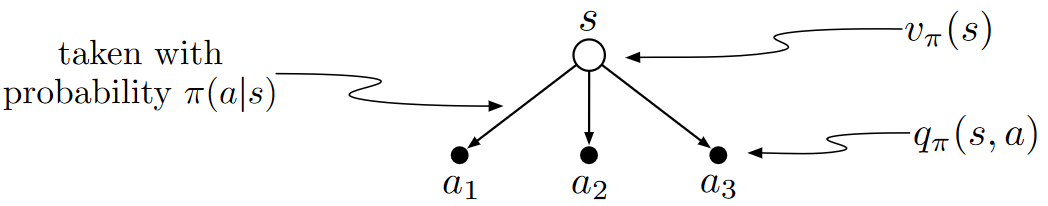
\includegraphics[width=0.8\textwidth]{chapters_latex/figures/ex_03_18.png}
\end{center}

Give the equation corresponding to this intuition and diagram for the value at the root
node, $v_\pi(s)$, in terms of the value at the expected leaf node, $q_\pi(s,a)$, given $S_t = s$. This
equation should include an expectation conditioned on following the policy, $\pi$. Then give
a second equation in which the expected value is written out explicitly in terms of $\pi(a|s)$
such that no expected value notation appears in the equation.

\subsubsection*{Solution:}

\[
    v_\pi(s)= \mathbb{E}_{\pi} \left[q_\pi(s,a) | S_t = s \right]
\]

\[
    v_\pi(s)= \sum_a \pi(a|s) q_\pi(s,a)
\]

\subsection*{Exercise 3.19} The value of an action, $q_\pi(s,a)$, depends on the expected next reward and
the expected sum of the remaining rewards. Again we can think of this in terms of a
small backup diagram, this one rooted at an action (state-action pair) and branching to
the possible next states:

\begin{center}
    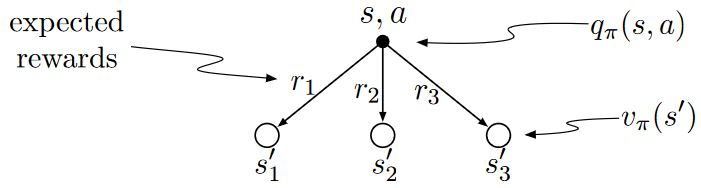
\includegraphics[width=0.6\textwidth]{chapters_latex/figures/ex_03_19.png}
\end{center}

Give the equation corresponding to this intuition and diagram for the action value,
$q_\pi(s,a)$, in terms of the expected next reward, $R_{t+1}$, and the expected next state value,
$v_\pi(S_{t+1})$, given that $S_t = s$ and $A_t = a$. This equation should include an expectation but
not one conditioned on following the policy. Then give a second equation, writing out the
expected value explicitly in terms of $p(s',r|s,a)$ defined by (3.2), such that no expected
value notation appears in the equation. 

\subsubsection*{Solution:}

\[
    q_\pi(s, a)= \mathbb{E} \left[R_{t+1} + \gamma v_\pi(S_{t+1}) | S_t = s, A_t = a \right]
\]

\[
    q_\pi(s, a)= \sum_{s',r} p(s',r|s,a) \left( r + \gamma v_\pi(s') \right)
\]


\subsection*{Exercise 3.20}
Draw or describe the optimal state-value function for the golf example.

\subsubsection*{Solution:}
Use the putter when on the green, use the driver in the other cases.
\begin{center}
    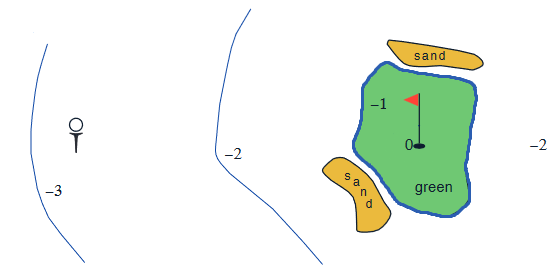
\includegraphics[width=0.6\textwidth]{chapters_latex/figures/ex_03_20.png}
\end{center}

\subsection*{Exercise 3.21} 
Draw or describe the contours of the optimal action-value function for putting,
$q_*(s, \text{putter})$, for the golf example.

\subsubsection*{Solution:}
$q_*(s, \text{putter})$ is equal to $1 + v_*(s')$ where $s'$ is the new location of the ball. If the ball arrives at the green, the next action should be using a putter, else the agent should use a driver.
\begin{center}
    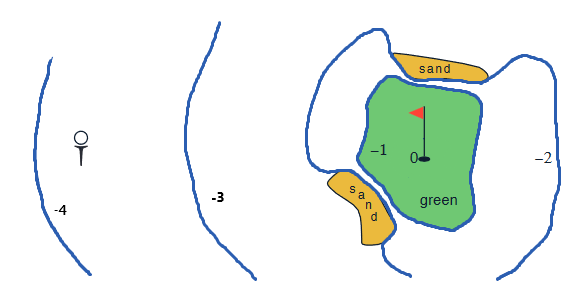
\includegraphics[width=0.6\textwidth]{chapters_latex/figures/ex_03_21.png}
\end{center}

\subsection*{Exercise 3.22}
Consider the continuing MDP shown to the
right. The only decision to be made is that in the top state,
where two actions are available, left and right. The numbers
show the rewards that are received deterministically after
each action. There are exactly two deterministic policies,
$\pi_\text{left}$ and $\pi_\text{right}$. What policy is optimal if  $\gamma = 0$? If  $\gamma = 0.9$?
If  $\gamma = 0.5$?
\begin{center}
    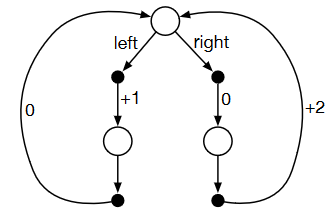
\includegraphics[width=0.6\textwidth]{chapters_latex/figures/ex_03_22.png}
\end{center}

\subsubsection*{Solution:}

After 2 actions the state will return to the original state, so $R_n = R_{n+2}$

\[
G_t = R_{t+1} + \gamma R_{t+2} + \gamma^2 G_t
\]

\[
(1 - \gamma^2) G = R_{t+1} + \gamma R_{t+2}
\]

\[
G_t = \frac{R_{t+1} + \gamma R_{t+2}}{1 - \gamma^2}
\]

$\pi_{\text{right}}$:   $G_t = \frac{2 \gamma}{1 - \gamma^2} $

$\pi_{\text{left}}$:   $G_t = \frac{1}{1 - \gamma^2} $

The optimal policy maximizes the value function, and because there is no stochasticity, $G_t = v_{\pi}(s)$.

If $(2\gamma > 1)$, going right is the optimal policy, while in the case of $(2\gamma < 1)$, going left is optimal.

For $(\gamma = 0)$: left is the optimal policy.

For $(\gamma = 0.9)$: right is the optimal policy.

For $(\gamma = 0.5)$: both policies are optimal.

\subsection*{Exercise 3.23}
Give the Bellman equation for $q_*$ for the recycling robot.

\subsubsection*{Solution:}

\begin{align*}
    q_*(\text{high}, \text{search}) &= r_\text{search} + \gamma \left( \alpha \max_a q_*(\text{high}, a) + (1 - \alpha) \max_a q_*(\text{low}, a) \right) \\
    q_*(\text{high}, \text{wait}) &= r_\text{wait} + \gamma \max_aq_*(\text{high}, a) \\
    q_*(\text{low}, \text{search}) &= \beta \left( r_\text{search} + \gamma  \max_a q_*(\text{low}, a) \right) \\
    &\quad + (1 - \beta) \left(-3 + \max_a q_*(\text{high}, a) \right) \\
    q_*(\text{low}, \text{wait}) &= r_\text{wait} + \gamma \max_aq_*(\text{low}, a) \\
    q_*(\text{low}, \text{recharge}) &= \gamma \max_aq_*(\text{high}, a)
\end{align*}

\subsection*{Exercise 3.24}
Figure 3.5 gives the optimal value of the best state of the gridworld as
24.4, to one decimal place. Use your knowledge of the optimal policy and (3.8) to express
this value symbolically, and then to compute it to three decimal places. 

\subsubsection*{Solution:}

\[
G_t = 10 + 0 + 0 + 0 + 0 + 0.9^5 \cdot G_t
\]
\[
G_t = \frac{10}{1-0.9^5} = 24.419
\]


\subsection*{Exercise 3.25}
Give an equation for $v_*$ in terms of $q_*$.

\subsubsection*{Solution:}

\[
v_*(s) = \max_a q_*(s,a)
\]

\subsection*{Exercise 3.26}
Give an equation for $q_*$ in terms of $v_*$ and the four-argument $p$.

\subsubsection*{Solution:}

\[
q_*(s,a) = \sum_{s', r} p(s', r |s, a)  \left( r + \gamma v_*(s') \right)
\]

\subsection*{Exercise 3.27}
Give an equation for $\pi_*$ in terms of $q_*$.

\subsubsection*{Solution:}

\[
\pi_*(a|s) =
    \begin{cases}
        1,  & \text{if } a = \argmax_a q_*(s,a)\\
        0,  & \text{else}
    \end{cases}
\]


\subsection*{Exercise 3.28}
Give an equation for $\pi_*$ in terms of $v_*$ and the four-argument $p$.

\subsubsection*{Solution:}

\[
\pi_*(a|s) =
    \begin{cases}
        1,  & \text{if } a = \argmax_a \sum_{s', r} p(s', r |s, a)  \left( r + \gamma v_*(s') \right)\\
        0,  & \text{else}
    \end{cases}
\]

\subsection*{Exercise 3.29}
Rewrite the four Bellman equations for the four value functions ($v_\pi$, $v_*$, $q_\pi$, $q_*$)
in terms of the three argument function $p$ (3.4) and the two-argument function $r$ (3.5).

\subsubsection*{Solution:}

\[
q_\pi(s,a) = r(s,a) + \gamma \sum_{s',a'} p(s'|s,a) \pi(a'|s') q _\pi(s',a')
\]

\[
    q_*(s,a) = r(s,a) + \gamma  \sum_{s'} p(s'|s,a) \max_{a'} \pi(a'|s') q _*(s',a')
\]

\[
    v_\pi(s) = \sum_a \pi(a|s) \left( r(s,a) + \gamma \sum_{s'} p(s'|s,a) v_\pi(s') \right) 
\]

\[
    v_*(s) = \max_a  r(s,a) + \gamma \sum_{s'} p(s'|s,a) v_*(s') 
\]